% ============================================================
%  Section 5 --- Résultats des hypothèses
% ============================================================

\section{Résultats}
\label{sec:results}

Les hypothèses sont évaluées sur le split test (45 épisodes, 15 scénarios) avec
le split val (45 épisodes) réservé à la sélection des hyperparamètres.
La robustesse est estimée sur 5 graines aléatoires indépendantes (42, 123, 456, 789, 1337),
chacune produisant un réentraînement complet de l'encodeur et du réseau siamois.
Les intervalles de confiance à 95\,\% sur l'AUROC sont obtenus par bootstrap
($n = 1000$ rééchantillonnages).

\subsection{H1 --- Structurabilité des embeddings}
\label{sec:h1}

\paragraph{Protocole.}
L'hypothèse H1 teste si les embeddings STGCN après typage siamois forment des clusters
exploitables dans l'espace latent, mesurés par le score de silhouette en held-out.
Le seuil de 0.3 est le minimum recommandé par Kaufman \& Rousseeuw \cite{kaufman1990}
pour une structure de clustering considérée comme significative.
Le nombre de clusters $K$ est sélectionné par maximum de silhouette sur val via un
sweep $K \in [5, 20]$ (gap statistic \cite{tibshirani2001} utilisée comme critère complémentaire).
Les labels val et test sont assignés par plus proche centroïde depuis les centroides train.

\paragraph{Résultats.}

\begin{table}[h]
\centering
\caption{Silhouette score par graine (seuil de PASS : $\geq 0.3$).}
\label{tab:h1_multiseed}
\begin{tabular}{cccccc}
\toprule
\textbf{Graine} & \textbf{sil\_val} & \textbf{sil\_test} & \textbf{K} & \textbf{H1} \\
\midrule
42   & 0.470 & 0.414 & 10 & \checkmark \\
123  & 0.624 & 0.662 & 10 & \checkmark \\
456  & 0.574 & 0.461 & 10 & \checkmark \\
789  & 0.466 & 0.469 & 10 & \checkmark \\
1337 & 0.545 & 0.591 & 11 & \checkmark \\
\midrule
\textbf{Agrégé} & $0.536 \pm 0.061$ & $\mathbf{0.519 \pm 0.092}$ & $10 \pm 0.7$ & \textbf{5/5} \\
\bottomrule
\end{tabular}
\end{table}

\textbf{H1 \checkmark{} PASS} : silhouette test $= 0.519 \pm 0.092$ sur 5 graines,
minimum $= 0.414 \gg 0.3$ (seuil de Kaufman \& Rousseeuw).
$K = 10$ clusters stable (écart-type $= 0.7$).

Les types de pannes sont structurellement séparables dans l'espace latent STGCN.
Cette séparabilité est le résultat du couplage entre la convolution spatiale sur $G(t)$ ---
qui encode la propagation des effets dans le graphe d'appel --- et le typage contrastif,
qui rapproche les épisodes de même scénario et éloigne les épisodes de scénarios différents.
L'analyse NMI (NMI cluster $\leftrightarrow$ scénario $= 0.518$, pureté moyenne $= 0.503$)
confirme un alignement modéré avec les labels Chaos Mesh, ce qui est attendu pour un
clustering non supervisé sur 15 scénarios distincts.

\begin{figure}[h]
\centering
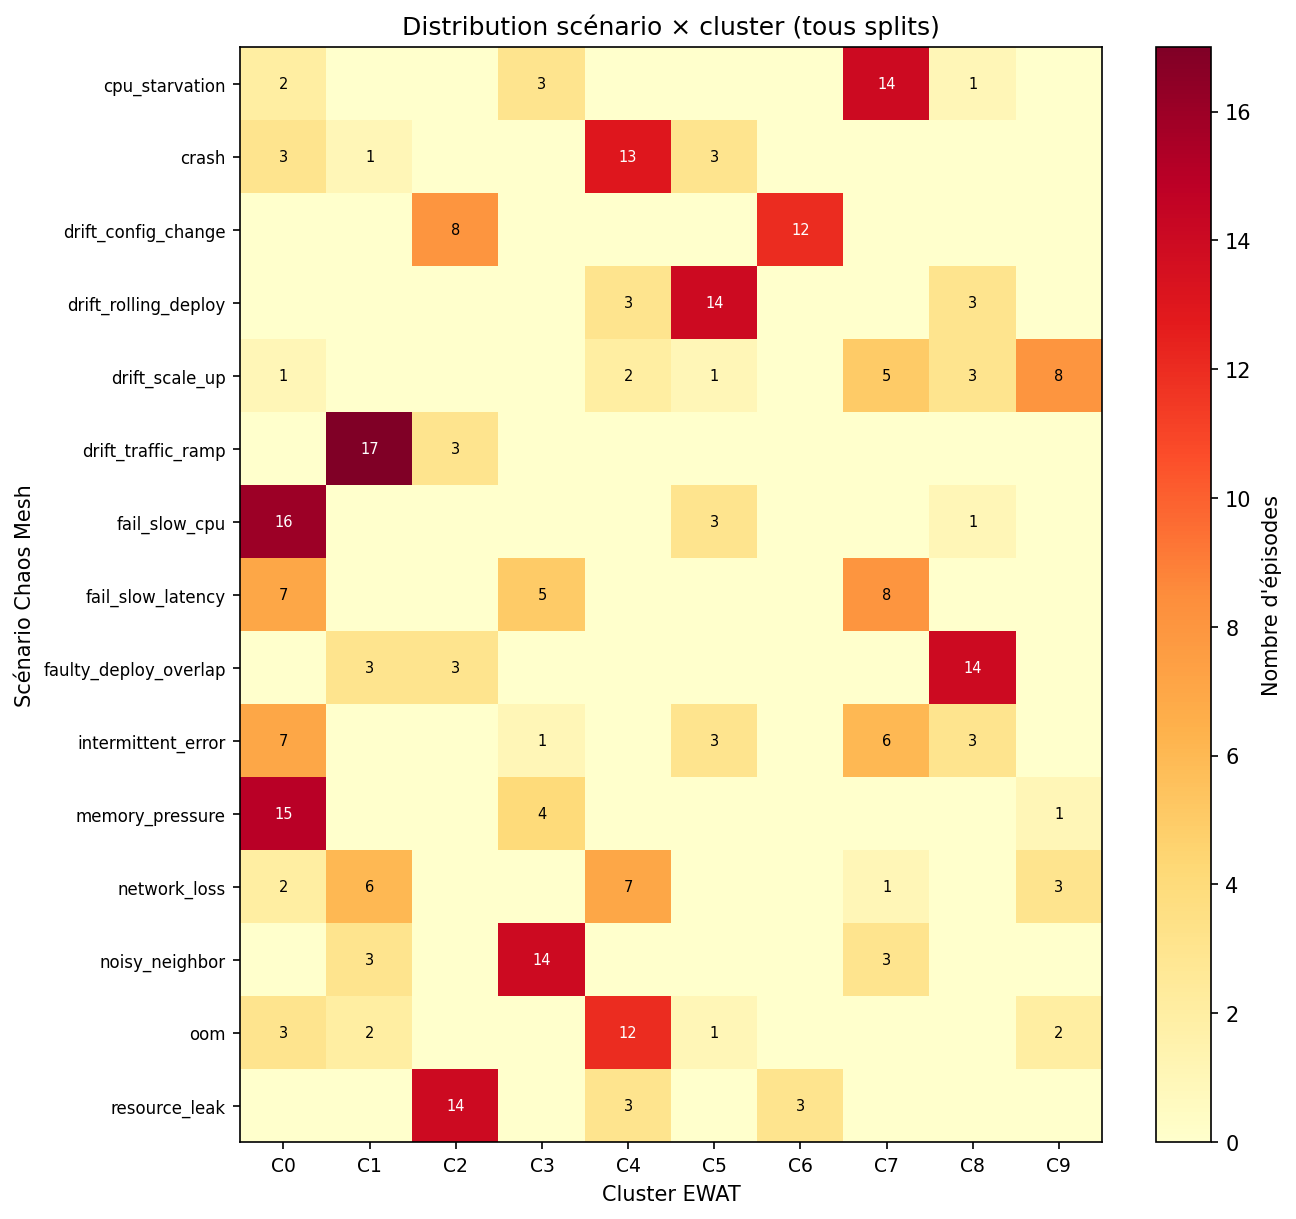
\includegraphics[width=0.78\linewidth]{figures/scenario_cluster_heatmap.png}
\caption{Distribution des épisodes par scénario Chaos Mesh et par cluster (15\,$\times$\,10).
  Chaque colonne représente un cluster ; chaque ligne un scénario.
  La diagonale dominante confirme la structure : la plupart des scénarios sont
  concentrés dans 1--2 clusters.}
\label{fig:cluster_heatmap}
\end{figure}

\subsection{H2a --- Séparabilité du drift par look-through}
\label{sec:h2a}

\paragraph{Protocole.}
L'hypothèse H2a compare le mécanisme look-through MMD-RFF à un seuil simple sur le même
signal. L'évaluation est conduite en mode streaming temporel sur les 45 épisodes test
(DriftDetector avec \texttt{post}=3 steps de confirmation).
Le test de Student unilatéral apparié teste si le FPR sur anomalie est réduit par
le look-through à rappel drift constant.

\paragraph{Résultats.}

\begin{table}[h]
\centering
\caption{Look-through vs.\ seuil simple --- test set (45 épisodes).}
\label{tab:h2a}
\begin{tabular}{lcc}
\toprule
\textbf{Métrique} & \textbf{Look-through} & \textbf{Seuil simple} \\
\midrule
TPR drift (drift $\to$ drift)             & 0.42 & \textbf{0.67} \\
FPR anomalie (anomalie $\to$ drift)       & 0.67 & 0.73 \\
$p$-value (Student unilatéral, FPR)       & \multicolumn{2}{c}{$0.27$} \\
\bottomrule
\end{tabular}
\end{table}

\textbf{H2a \xmark{} FAIL} ($p = 0.27 > 0.05$).
Le mécanisme look-through n'apporte pas de réduction significative du FPR sur anomalie.

\paragraph{Interprétation.}
La cause est identifiée et quantifiable. Chaque épisode dure $\approx 21$ steps.
Le DriftDetector nécessite un warm-up de $\approx 8$ steps avant d'avoir une fenêtre
de référence stable, et le mécanisme de confirmation temporelle requiert $3$--$6$ steps
supplémentaires. Il ne reste donc que $\approx 7$ steps utiles par épisode --- soit 33\,\%
de la durée totale --- pour que le look-through opère. Sur cette fenêtre réduite,
la puissance statistique est insuffisante pour atteindre $p < 0.05$.

Ce résultat est complété par une évaluation du look-through sur les embeddings STGCN
(H2a bis) : FPR$_\text{lt} = 0.788 >$ baseline $= 0.667$, $p = 0.978$. Les embeddings
STGCN capturent le \emph{type} de panne (H1 validée), pas le \emph{régime}
drift/anomalie --- ce qui est cohérent avec leur conception : le réseau siamois
est entraîné sur des paires de scénarios, sans supervision sur la distinction
drift/anomalie.

Ce résultat négatif est honnête et exploitable : il ne remet pas en cause la conception
du mécanisme, mais définit précisément la contrainte de données à lever dans ewat\_v4
($\geq 40$ steps par épisode).

\subsection{H2b --- Identification du régime $\theta_{\text{drift} \cap \text{anomaly}}$}
\label{sec:h2b}

\paragraph{Protocole.}
H2b teste si le cluster C8 (\texttt{faulty\_deploy\_overlap}, régime
$\theta_{\text{drift} \cap \text{anomaly}}$) présente simultanément un flag drift
et une alerte précurseur à une fréquence significativement supérieure aux clusters
de drift pur (C5 + C6 + C9 poolés). Le critère formel (overlap $> 30$\,\%) est
complété par un critère strict : test Fisher exact et analyse de sensibilité au seuil.

\paragraph{Résultats --- critère formel.}
L'overlap drift+alerte dépasse 30\,\% pour les 10/10 clusters, y compris pour C5, C6
et C9 (drifts purs). Ce résultat est trivial : le DriftDetector, avec une fenêtre de
5 steps, déclenche sur quasi tous les épisodes quel que soit leur type, et les classifieurs
précurseurs (seuil 0.4) déclenchent également très fréquemment.
C8 présente : drift\% $= 0.85$, alerte\% $= 0.92$, overlap\% $= 0.77$, cohérent avec
$\theta_{\text{drift} \cap \text{anomaly}}$, mais sans contrôle statistique sur les drifts purs.

\paragraph{Résultats --- critère strict (analyse de sensibilité).}

\begin{table}[h]
\centering
\caption{Sensibilité du critère d'overlap.}
\label{tab:h2b_sensitivity}
\begin{tabular}{cc}
\toprule
\textbf{Seuil} & \textbf{Clusters PASS} \\
\midrule
$> 30$\,\% & 10/10 \\
$> 50$\,\% & 10/10 \\
$> 70$\,\% & 6/10 (C0, C1, C3, C5, C8, C9) \\
$> 90$\,\% & 1/10 (C1 uniquement) \\
\bottomrule
\end{tabular}
\end{table}

Fisher exact C8 vs.\ drift pur (C5+C6+C9 poolés) :
$\text{OR} = 1.48$, $p = 0.35$ --- \textbf{non significatif}.

\paragraph{Résultats --- timing.}
L'analyse temporelle révèle que l'alerte précurseur \emph{précède} le flag drift dans
85--100\,\% des épisodes (timing gap médian $< 0$ pour tous les clusters).
Le DriftDetector est un indicateur \emph{tardif} : il confirme une transition de régime
déjà détectée par les précurseurs. Cela est cohérent avec sa mécanique : la confirmation
temporelle (3--6 steps) s'ajoute au warm-up (8 steps), totalisant jusqu'à 14 steps de
délai depuis l'injection.

\paragraph{Interprétation.}
H2b PASS trivial renforce le diagnostic de H2a : le DriftDetector est trop sensible sur
des épisodes de 21 steps pour discriminer drift et anomalie. La conclusion est la même
dans les deux cas --- limitation de données, pas défaut de conception. Sur ewat\_v4
($\geq 40$ steps), la fenêtre de confirmation sera suffisante pour tester H2b
avec un contrôle statistique valide.

\subsection{H3 --- Prédictibilité des précurseurs typés}
\label{sec:h3}

\paragraph{Protocole.}
Pour chaque type $C_i$, le classifieur $f_i$ est entraîné sur train, $k^*_i$ est sélectionné
par maximum d'AUROC sur val, et l'AUROC est rapporté sur test. Les clusters avec
$n_\text{pos\_test} < 2$ sont exclus (AUROC non calculable).
Les IC à 95\,\% sont obtenus par bootstrap ($n = 1000$).

\paragraph{Résultats.}

\begin{table}[h]
\centering
\caption{AUROC précurseur par type de cluster (graine 42, k* sur val).}
\label{tab:h3}
\begin{tabular}{llccc}
\toprule
\textbf{Type} & \textbf{Scénario dominant} & \textbf{$k^*$} & \textbf{AUROC test} & \textbf{IC 95\,\%} \\
\midrule
C0 & fail\_slow\_cpu       & 6  & 0.973 & [0.906, 1.000] \\
C1 & drift\_traffic\_ramp  & 6  & 0.992 & [0.953, 1.000] \\
C2 & resource\_leak        & 6  & 0.945 & [0.865, 1.000] \\
C3 & noisy\_neighbor       & 2  & 0.794 & [0.636, 0.930] \\
C4 & crash                 & 2  & 1.000 & [1.000, 1.000] \\
C5 & drift\_rolling\_deploy& 6  & 0.977 & [0.909, 1.000] \\
C6 & drift\_config\_change & 2  & NaN   & $n_\text{pos} < 2$ \\
C7 & cpu\_starvation       & 6  & 0.992 & [0.966, 1.000] \\
C8 & faulty\_deploy\_overlap& 10 & 0.962 & [0.895, 1.000] \\
C9 & drift\_scale\_up      & 2  & NaN   & $n_\text{pos} < 2$ \\
\bottomrule
\end{tabular}
\end{table}

\textbf{H3 \checkmark{} PASS} : AUROC moyen $= 0.973 \pm 0.012$ (5 graines),
8/10 types prédictibles. C6 et C9 : NaN par insuffisance de positifs ($n_\text{pos} = 1$).

L'horizon optimal $k^* = 6$ steps (3\,min) pour 5 types sur 8 établit un
\textbf{lead time opérationnel de 3\,min} --- temps suffisant pour déclencher une
procédure de rollback sur Kubernetes avant que la dégradation n'atteigne les SLOs utilisateurs.
C3 présente l'IC le plus large ([0.636, 0.930], $n_\text{pos} = 3$),
reflétant la faible représentation de \texttt{noisy\_neighbor} dans le test set
(Figure~\ref{fig:auroc_h3}).

\begin{figure}[h]
\centering
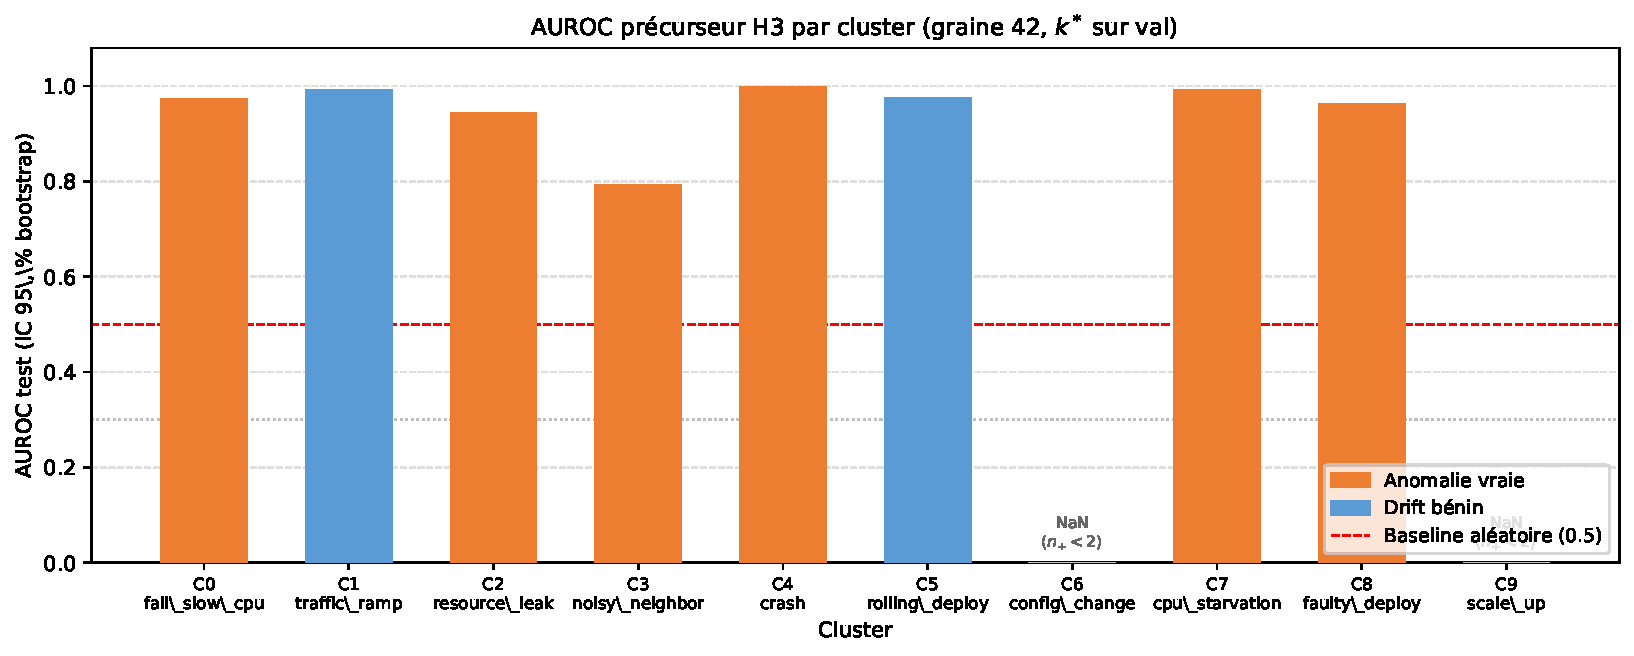
\includegraphics[width=0.92\linewidth]{figures/auroc_h3_per_cluster.pdf}
\caption{AUROC précurseur par cluster (graine 42, $k^*$ sélectionné sur val).
  Barres orange = anomalies, bleu = drifts bénins.
  Les barres d'erreur représentent les IC 95\,\% bootstrap.
  C6 et C9 (gris) : NaN, $n_\text{pos} = 1$.}
\label{fig:auroc_h3}
\end{figure}

\begin{table}[h]
\centering
\caption{Robustesse H3 sur 5 graines.}
\label{tab:h3_multiseed}
\begin{tabular}{cccc}
\toprule
\textbf{Graine} & \textbf{AUROC moyen} & \textbf{Types PASS} & \textbf{H3} \\
\midrule
42   & 0.951 & 8/10 & \checkmark \\
123  & 0.984 & 7/10 & \checkmark \\
456  & 0.981 & 7/9  & \checkmark \\
789  & 0.977 & 8/11 & \checkmark \\
1337 & 0.972 & 7/10 & \checkmark \\
\midrule
\textbf{Agrégé} & $\mathbf{0.973 \pm 0.012}$ & 7--8/K & \textbf{5/5} \\
\bottomrule
\end{tabular}
\end{table}

La variance inter-graines est faible (écart-type $= 0.012$), ce qui confirme la robustesse
des précurseurs aux initialisations aléatoires du pipeline. L'AUROC moyen reste supérieur
à $0.95$ pour toutes les graines --- bien au-dessus du seuil de falsification ($0.5$).

\subsection{Système d'alerte --- comparaison avec le z-score}
\label{sec:alerts_results}

\begin{table}[h]
\centering
\caption{Comparaison EWAT vs.\ baseline z-score (test set, 45 épisodes).
  IC\,95\,\% Wilson sur Détection ($n=33$ anomalies) et FA ($n=12$ drifts).}
\label{tab:alerts}
\begin{tabular}{lcccc}
\toprule
\textbf{Méthode} & \textbf{Détection} & \textbf{IC\,95\,\%} & \textbf{FA drift} & \textbf{Lead time} \\
\midrule
z-score ($\sigma \in [2.0, 3.5]$) & 100\,\% & --- & 100\,\% & 2.5\,min \\
EWAT seuil 0.3 & 100\,\% & --- & 100\,\% & 4.6\,min \\
EWAT seuil 0.5 & 78.8\,\% & [62.0, 89.4]\,\% & 100\,\% & 3.9\,min \\
\textbf{EWAT seuil 0.7} & \textbf{57.6\,\%} & \textbf{[40.8, 72.8]\,\%} & \textbf{8.3\,\%} & \textbf{3.0\,min} \\
\bottomrule
\end{tabular}
\end{table}

\begin{table}[h]
\centering
\caption{IC\,95\,\% Wilson sur la FA drift au seuil 0.7 ($n_\text{drift}=12$, 1 fausse alarme).}
\label{tab:alerts_ci_fa}
\begin{tabular}{lccc}
\toprule
\textbf{Seuil} & \textbf{FA observée} & \textbf{IC\,95\,\% Wilson} & \textbf{$n_\text{drift}$} \\
\midrule
0.5 & 100\,\% & --- & 12 \\
0.7 & 8.3\,\% & [1.5, 35.4]\,\% & 12 \\
\bottomrule
\end{tabular}
\end{table}

L'apport principal d'EWAT par rapport à la baseline z-score est la réduction du taux de
fausses alarmes sur les drifts bénins. Quel que soit le seuil $\sigma \in [2.0, 3.5]$,
le z-score déclenche une alerte sur 100\,\% des épisodes de drift bénin --- il ne dispose
d'aucun mécanisme pour distinguer un déploiement progressif d'une vraie anomalie.
Ce comportement est \emph{structurel} : un z-score univarié mesure l'écart à la moyenne
glissante de chaque métrique indépendamment. Un drift bénin et une anomalie réelle
produisent des déviations statistiques comparables sur les mêmes métriques (latence,
taux d'erreur) car le z-score n'a accès ni à la topologie du graphe $G(t)$, ni au
contexte des régimes $\theta(t)$. Réduire $\sigma$ augmente les fausses alarmes sur
données normales ; l'augmenter fait manquer les vraies pannes.
Aucun choix de seuil ne résout le problème de discrimination drift\,/\,anomalie.

EWAT au seuil 0.7 réduit ce taux à 8.3\,\% (1 épisode de drift sur 12 produit une alerte),
soit une réduction d'un facteur 12, tout en maintenant un lead time de 3.0\,min.
Ce gain est obtenu grâce au typage contrastif : les clusters de drift (C5, C6, C9) ont
des précurseurs entraînés spécifiquement sur les signatures de drift bénin, ce qui permet
à l'AlertAssembler de distinguer ces signatures des anomalies réelles.

La détection d'anomalies réelles au seuil 0.7 est de 57.6\,\% [40.8, 72.8]\,\% --- en deçà
des 100\,\% du z-score. Ce trade-off est explicite et contrôlable par le seuil : le seuil 0.3
retrouve 100\,\% de détection avec 100\,\% de FA, tandis que le seuil 0.7 offre le meilleur
équilibre FA/détection sur les données disponibles.

\textbf{Note de prudence.}
La FA de 8.3\,\% au seuil 0.7 repose sur un seul épisode de drift déclenché sur douze
($n_\text{drift} = 12$). L'IC Wilson à 95\,\% est [1.5, 35.4]\,\% : la borne haute à 35\,\%
interdit toute extrapolation ferme. Ce résultat est indicatif du comportement du pipeline
sur ewat\_v3 ; sa confirmation sur ewat\_v4 ($n_\text{drift}$ plus grand) est nécessaire
pour établir une garantie opérationnelle.

\begin{figure}[h]
\centering
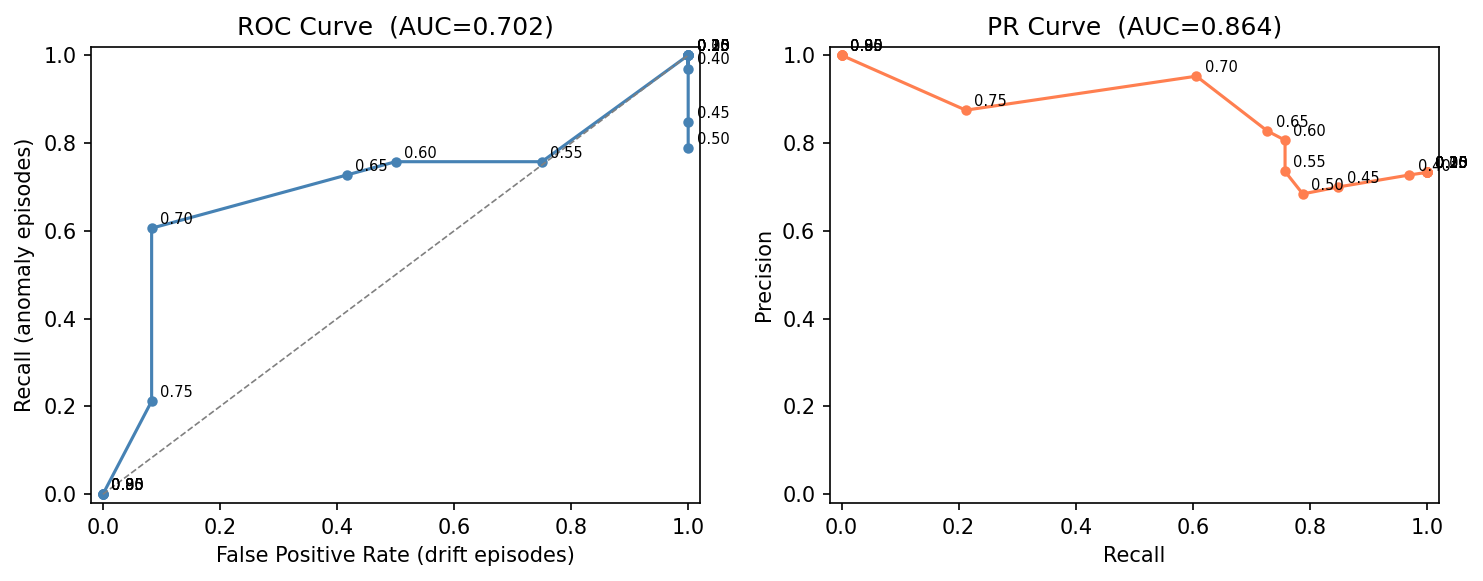
\includegraphics[width=0.75\linewidth]{figures/roc_pr_curve.png}
\caption{Courbes ROC et PR de l'AlertAssembler (test set, 45 épisodes).
  La courbe ROC illustre le trade-off FA/détection en fonction du seuil.}
\label{fig:roc_pr}
\end{figure}
